\documentclass[a4paper, titlepage]{article}
\usepackage{cite}
\usepackage{listings}
\usepackage{graphicx}
\usepackage{color}
\usepackage{pbox}
\usepackage{hyperref}


\begin{document}
\newcounter{commentcount}
\newcommand{\currcmt}{\value{commentcount}}

\newcommand{\comment}[2]{#1\marginpar{#2}}
\newcommand{\ggcomment}[1]{\comment{\textcolor{red}{$^{\arabic{commentcount}}$}}{\textcolor{red}{$^{\arabic{commentcount}}$GG: #1}}\stepcounter{commentcount}}
\newcommand{\vtcomment}[1]{\comment{\textcolor{blue}{$^{\arabic{commentcount}}$}}{\textcolor{blue}{$^{\arabic{commentcount}}$VT: #1}}\stepcounter{commentcount}}
% dafny and tacny code
\newcommand{\dcode}[1]{\texttt{#1}}

\title{
Search space reduction for Dafny tactics
}

\author{Vytautas Tumas}

\maketitle
\tableofcontents

\section{Tools}
The datasets were reduced with the AWK script provided in the coursework description and the algorithms were implemented in Python.
\section{Histograms}
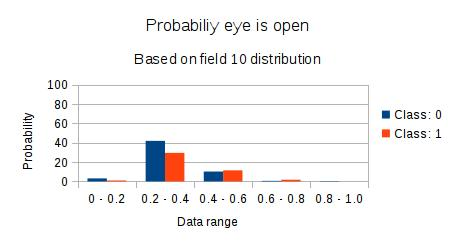
\includegraphics[scale=0.5]{eeg/field_10}
\section{Nearest Neighbour}


\end{document}